\subsubsection{Objective}
The third research question investigates how the installation dates and operational periods of weather stations affect data availability over time and across Austrian regions and elevation zones. The goal is to identify spatial and temporal coverage gaps, also referred to as ``data deserts,'' that could affect the interpretation of long-term climate analyses.

\subsubsection{Methodology}

To address this question, the implementation proceeded in two main steps:

\begin{enumerate}
  \item \textbf{Metadata-Based Coverage Matrix:}  
    Using station metadata (installation and deactivation dates), a year-by-year activity matrix was constructed from 1960 to 2025 using a cross join. Active periods were filtered, and each station was assigned to one of five elevation bands:
    \begin{itemize}
      \item 0--499\,m (Lowland)
      \item 500--999\,m (Upland)
      \item 1000--1499\,m (Lower Alps)
      \item 1500--1999\,m (Alpine)
      \item 2000+\,m (High Alpine)
    \end{itemize}
    Aggregated counts by year, elevation zone, and federal state provided a theoretical view of station coverage.

  \item \textbf{Real Measurement-Based Coverage:}  
    To verify actual data presence, the climate dataset was filtered to include only records with at least one valid measurement. These were grouped using the same schema as the metadata-based approach.
\end{enumerate}

To keep the report focused, only the Lower Alps zone is discussed in detail as it highlights key patterns.

\subsubsection{Results and Interpretation}

\paragraph{Figure~\ref{fig:coverage_meta_loweralps}: Metadata-Based Coverage (Lower Alps)}  
The heatmap shows that while Tyrol and Salzburg maintained a consistent network of 10--30 active stations yearly since the 1970s, regions like Lower Austria and Upper Austria exhibit almost no presence in this elevation zone. This confirms topographic disparities in historical climate monitoring.

\begin{figure}[ht]
  \centering
    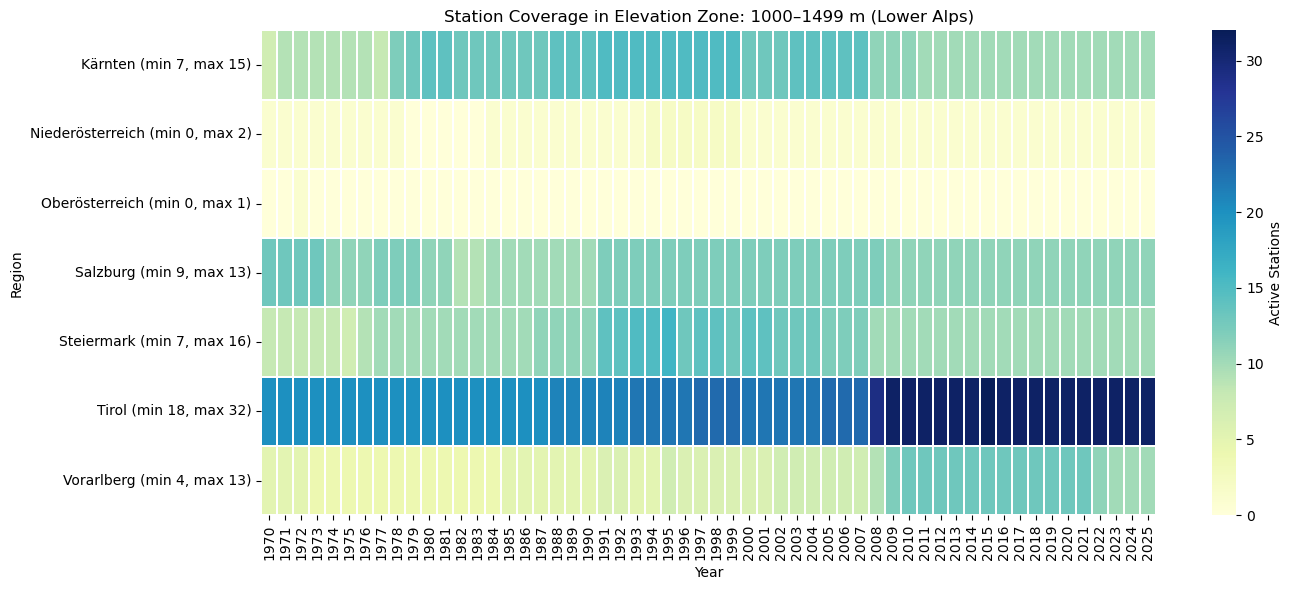
\includegraphics[width=0.45\textwidth]{img/coverage_zone_loweralps_meta.png}
    \caption{Metadata-based station coverage in elevation zone: 1000--1499\,m (Lower Alps)}
    \label{fig:coverage_meta_loweralps}
\end{figure}

\paragraph{Figure~\ref{fig:coverage_real_loweralps}: Actual Measurement-Based Coverage (Lower Alps)}  
The second heatmap confirms that actual measurement coverage aligns well with the metadata. Again, Tyrol is best represented, while several eastern federal states have minimal or no data-producing stations in this zone.

\begin{figure}[ht]
  \centering
    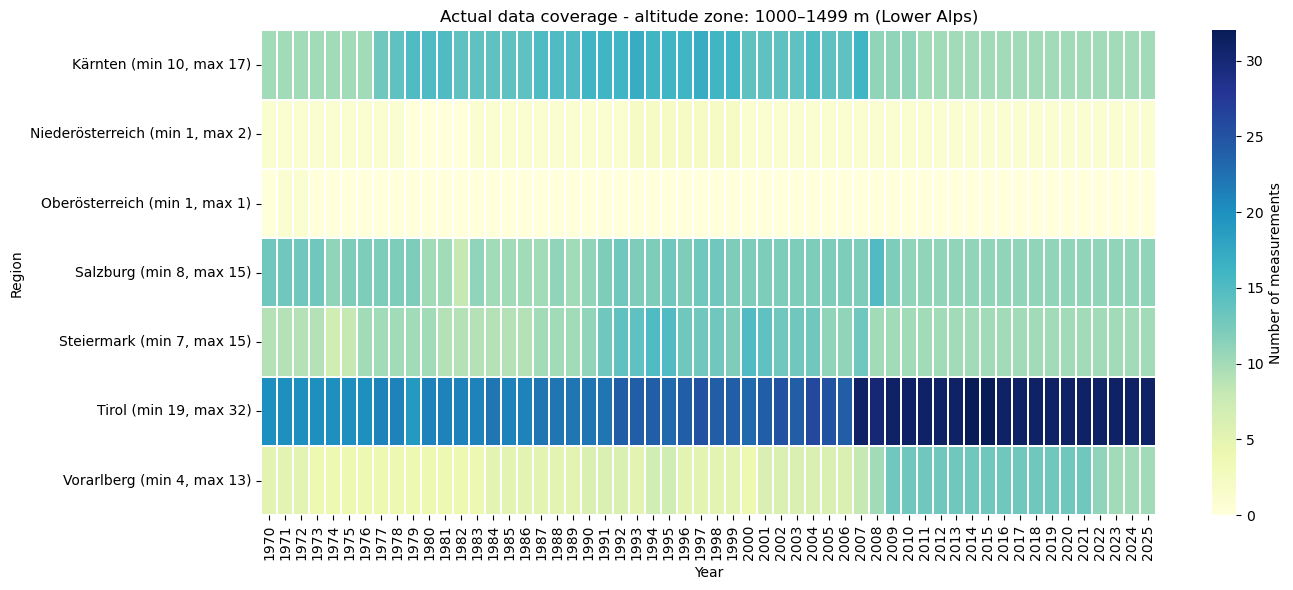
\includegraphics[width=0.45\textwidth]{img/data_coverage_loweralps.png}
    \caption{Actual measurement-based coverage in elevation zone: 1000--1499\,m (Lower Alps)}
    \label{fig:coverage_real_loweralps}
\end{figure}

\subsubsection{Conclusion}
Both metadata and actual measurement coverage confirm consistent long-term gaps in mid-altitude mountain zones across eastern Austrian regions. Western alpine states such as Tyrol provide dense and uninterrupted coverage. The stepwise implementation, beginning with metadata modeling and validated through real data filtering, proves effective in uncovering structural weaknesses in historical climate data availability.
